\chapter{Capacidade de Armazenamento}

Vimos que a geometria do disco rígido envolve trilhas, setores e cilindros e que em cada setor do disco cabem 512 bytes de informação. Para identificar a capacidade de armazenamento de um disco basta utilizar a geometria, se um disco tem 2.448 cilindros, 16 lados (ou ``cabeças'' de leitura) e 63 setores por trilha, terá 2.448 x 16 x 63 = 2.467.584 setores. Logo, se multiplicarmos a quantidade de setores pela quantidade de informação que cabe em cada setor teremos a capacidade total do disco, que no caso é de 1.263.403.008 bytes, e como cada KB tem 1.024 bytes, dividindo-se por 1.024 uma vez para identificar a quantidade de KB do disco, divide-se novamente para identificar a quantidade em MB e novamente para identificar a quantidade em GB. Sendo assim esse disco teria a capacidade real de 1.18 GB.

\chapter{FAT}

\section{FAT-16}

O sistema FAT (File Allocation Table), utiliza uma tabela de alocação de arquivos representando um mapa de utilização do disco, o que permite ao sistema operacional ser capaz de saber exatamente onde um determinado arquivo está armazenado.

A FAT possui várias posições para localização de arquivos no disco. Como cada posição na FAT-16 utiliza 16 bits, podemos ter, no máximo, 256 (16 \^ 2) = 65.536 posições na FAT.

\subsection{Tabela de Alocação}

Como em um setor cabem 512 bytes, teoricamente, só poderiamos ter discos de 65.536 x 512 bytes = 33.554.432 bytes = 32 MB. Por esse motivo, o sistema FAT-16 não trabalha com setores mas sim com unidades de alocação chamadas \emph{\textbf{clusters}}, que é um conjunto de setores.

\subsection{Cluster}

Ao invés de cada posição da FAT apontar para um setor, ela aponta para um cluster, podendo ser de 1, 2, 4 ou mais setores do disco. O tamanho do cluster é definido automaticamente pelo sistema operacional quando o disco é formatado, seguindo uma tabela.

Sendo o cluster a menor unidade a ser acessada pelo sistema operacional, os arquivos deverão ter obrigatoriamente tamanhos múltiplos do tamanho do cluster, o que significa que um arquivo de 100 KB em um disco rígido que utilize clusters de 8KB obrigatoriamente ocupará 13 clusters e não 12,5 como seria a divisão de 100 por 8. Isso daria um total de 104 KB, neste caso temos um \emph{\textbf{desperdício}} de 4 KB. Quanto maior o tamanho do cluster, maior o desperdício.

Esse espaço deixado pelo arquivo dentro do cluster é muito importante para a forense computacional, chamado de \textbf{Slack Space}. Esse espaço costuma ficar vestígio de arquivos manipulados no sistema. 

\begin{citacao}
  Forense em sistemas FAT-16 podem apontar grandes quantidades de informações em slack space.
\end{citacao}

Todo o espaço que de armazenamento que sobra de um cluster não é reutilizado para armazenar outro arquivo. \emph{Um cluster só pode ser utilizado por um arquivo.}

Uma limitação do FAT-16 é que ele só permite gerenciar discos de até 2 GB de partição.

\subsection{FAT-32}

Com o FAT-32 o tamanho do cluster é sensivelmente menor, fazendo com que haja bem menos desperdício, reduzindo o slack space. Permite, também, o uso de discos maiores, até 1 TB em uma partição.

\section{NTFS}

Esse sistema de arquivos permite que a menor unidade de alocação (512 bytes) possa ser usada como o próprio setor, evitando assim desperdício de espaço.

O sistema NTFS utiliza 64 bits para endereçar os dados em sua MFT (Master File Table - tabela de endereçamento). Com o uso de clusters de 64 KB o limite de dados pode chegar aos 256 TB. O tamanho do cluster é definido automaticamente pelo sistema operacional ou pela formatação de uma partição, podendo ir de 512 bytes a 64 KB, e também podendo ser definido pelo usuário em procedimentos específicos.

\begin{citacao}
  Durante o processo de formatação do disco, é criado o MBR (Master Boot Record). O MBR contém uma quantidade pequena de códigos executáveis chamada de ``master boot code'' e contém também a tabela de partição do disco. A tabela de partição contém um determinado número de campos para descrever a partição. Um desses campos é o System ID, que define o file system, como o NTFS, na partição. Para volumes NTFS o ID é 0x07. 
\end{citacao}

A figura \ref{fig:ntfs} demonstra a arquitetura do NTFS.

\begin{figure}[htb]
	\centering
	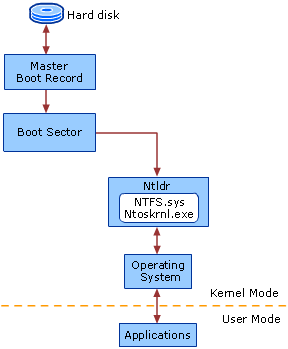
\includegraphics[width=0.8\textwidth]{sistemas_de_arquivos/fig/ntfs.png}
	\caption{Arquitetura do NTFS}
	\label{fig:ntfs}
\end{figure}

\newpage

O link \textbf{http://technet.microsoft.com/en-us/library/cc781134(v=ws.10).aspx} serve como referência para aprofundamento no NTFS.

\subsection{Tolerância a Falhas}

Para preservar os dados o NTFS utiliza um esquema de \emph{journaling}, um arquivo de log que indica falhas para posterior recuperação de dados. O log registra todas as ações que acontecem no sistema em relação aos arquivos. Quando um documento é criado, um espaço é alocado para ele, suas permissões são definidas, e assim por diante. Nesse meio tempo pode haver uma queda de energia e o espaço definido para o arquivo ser alocado, mas não utilizado. Quando o sistema operacional é reativado, ele consulta o arquivo de log para saber quais procedimentos não foram executados por completo e executa a ação correspondente para corrigir o problema.

\subsection{MFT - Master File Table}

A MFT tem praticamente a mesma finalidade da FAT, porém, funciona de uma forma diferente.

O MFT registra atributos de cada arquivo armazenado, consistindo em uma série de informações como por exemplo:

\begin{itemize}
	\item Nome do arquivo;
	\item Data da última modificação;
	\item Permissões; e
	\item Localização na unidade de armazenamento.
\end{itemize}

Cada entrada na MFT possui cerca de 2 KB, onde são armazenados o nome do arquivo e seus atributos, sobrando uma pequena área de dados que é usada para guardar o início do arquivo.

\begin{citacao}
  Em alguns casos, não é possível armazenar nem mesmo os atributos do arquivo, neste caso, os atributos são gravados em clusters no HD e na MFT ficam as entradas que apontam para os clusters.
\end{citacao}

\subsection{EFS}

O EFS é um recurso de criptografia permitindo uma maior proteção dos dados por criptografia utilizando chaves públicas. A principal vantagem é que o dono dos arquivos protegidos pode determinar quais usuários prodem acessá-los.

\section{ext3}

